% elements-of-flash-forth-5.tex
% PJ, 27-May-2013, 2017-02-05

\documentclass[12pt,a4paper]{article}
\usepackage[body={16cm,24cm}]{geometry}
\usepackage{graphicx}
% \usepackage{bytefield}
\usepackage{listings}
\pagestyle{headings}
\usepackage{textcomp}
\usepackage{hyperref}
\hypersetup{colorlinks=true,linkcolor=blue}

\lstset{basicstyle=\ttfamily, showstringspaces=false, identifierstyle=, keywordstyle=}
\lstset{numbers=left, numberstyle=\tiny, stepnumber=1, numbersep=5pt}
\newcommand{\code}[2]{
 \hrulefill
 \scriptsize
 \lstinputlisting{#2}
 \hrulefill
 \vspace{2em}
 \normalsize
}

%------------------------------------------------------------------
% a couple horizontal bars to delimit embedded code
% the width suits that set above and
% the mathmode eliminates spaces between the three elements
\newcommand{\topbar}{\ensuremath{
    \rule{0.1mm}{2.0mm} \rule[2.0mm]{159.5mm}{0.1mm} \rule{0.1mm}{2.0mm}
}}
\newcommand{\bottombar}{\ensuremath{
    \rule{0.1mm}{2.0mm} \rule{159.5mm}{0.1mm} \rule{0.1mm}{2.0mm}
}}

%------------------------------------------------------------------

\title{
    Elements of FlashForth 5.
}
\author{
    Mechanical Engineering Report 2017/01\\
    Peter Jacobs\thanks{peterj@mech.uq.edu.au}, 
    Pete Zawasky\thanks{PZEF Company -- Hardware and Software for Instrumentation and Control; pzawasky@pzef.net} and 
    Mikael Nordman\thanks{http://www.flashforth.com/; mikael.nordman@flashforth.com}\\
    School of Mechanical and Mining Engineering\\
    The University of Queensland.
}

\begin{document}
\maketitle

\begin{abstract}
This report is a remix of material from a number of Forth tutorials and references, 
adapted to the FlashForth environment.
It provides some examples and explanation of using FlashForth on a PIC18 microcontroller
while concentrating on the features of the language rather than the details of the
microcontroller hardware.
Following an introduction to the FlashForth interpreter, 
we look at adding our own word definitions to the dictionary and then explore
the manipulation of data values on the stack.
Flow of program control and more advanced defining words are also explored.
These defining words are convenient for making arrays.
Finally, strings and formatted numeric output are discussed.
\end{abstract}

\newpage
\tableofcontents

\cleardoublepage
\section{Introduction}
\label{sec:introduction}
%
Forth is an interesting mix of low-level access tools and language building tools.
It is effectively a small toolkit with which you construct a specialized dictionary of words
that work together to form your application code.
This tutorial will explore and explain the workings of the FlashForth toolkit
running on a Microchip PIC18 microcontroller
and complements the more hardware-oriented tutorial \cite{jacobs_2016a},
the FlashForth quick reference \cite{jacobs_2016b} and
the FlashForth website \cite{flashforth5}.
Our interest is in using Forth on the microcontroller in an embedded system,
such as a special-purpose signal timing device,
rather than as part of a general-purpose calculation on a personal computer.

\medskip
There are quite a number of good introductory tutorials \cite{brodie_1987a,noble_2001a}, 
course notes \cite{pelc_2011a},
and references \cite{conklin_rather_2007a} 
for programming in Forth on a desktop or laptop computer,
however, FlashForth running on a PIC18 microcontroller is a different environment.
In the following sections, we will follow closely J.~V.~Noble's tutorial \cite{noble_2001a}
for using Forth on a personal computer,
reusing many of his examples and explanations verbatim, 
while adapting the overall tutorial to the use of FlashForth on a microcontroller.

\newpage
\section{Getting started}
\label{sec:getting-started}
%
Although we will be using FlashForth on a PIC18 microcontroller, we communicate with it
using a serial terminal program running on a personal computer.
FlashForth comes with a couple of terminal programs (in Python and Tcl/Tk)
that have some conveniences when sending files to the microcontroller,
so we will start our interaction with one of those.
Starting the \verb!ff-shell.tcl! program in a normal terminal window
will start up the Tcl/Tk shell program.
Pressing the \fbox{ENTER $\hookleftarrow$} key a couple of times should get the display 
as shown in Figure\,\ref{fig:opening-screen}.
The \verb!ok<#,ram>! prompt indicates that the current base is ten,
for representing numbers in decimal format, 
and that the current context for making variables is static RAM, 
rather than the Flash memory and EEPROM that is also available in the microcontroller.

\begin{figure}[htb]
 \centering
 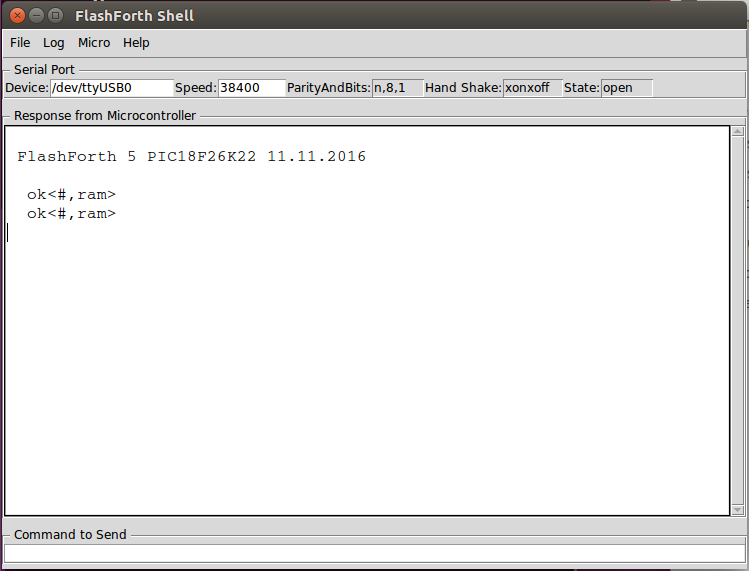
\includegraphics[width=0.9\textwidth]{../figs/ff5-start-screen-ff-shell-tcl.png}
 \caption{Opening screen using \texttt{ff-shell.tcl}.}
 \label{fig:opening-screen}
\end{figure}

\medskip
In contrast to Forth on a PC, FlashForth is case sensitive, with most predefined words 
being spelled with lower case.
Also, being intended for use in an embedded system, there is no command to exit the system.
FlashForth only stops when the power is removed or a reset occurs.

\newpage
\section{The interpreter}
\label{sec:interpreter}
%
FlashForth is an interactive programming language consisting of \textit{words}.
Forth words are the equivalent of subroutines or functions in other languages and are
executed by naming them.
Although FlashForth is interactive at its core, the user doesn't need to
interact with an embedded application if its top-level word is set to automatically
execute at power-up.

\medskip
Here is an example of executing a FlashForth word: \vspace{7pt} \\
\verb!hex! \fbox{$\hookleftarrow$} \verb!  ok<$,ram>! \vspace{7pt} \\
This executes the word that sets the base for representing numbers to 16, 
a format that you are likely to be familiar with
if you are a student of mechatronics or computing.
Note that both the text that your typed and the FlashForth response is shown
together, on either side of the Enter symbol \fbox{$\hookleftarrow$}.
For the moment, let's return to using decimal numbers: \vspace{7pt} \\
\verb!decimal! \fbox{$\hookleftarrow$} \verb!  ok<#,ram>! \vspace{7pt} \\

\medskip
Now, let's try something a bit more interesting by entering: \vspace{7pt} \\
\verb!2 17 + .! \fbox{$\hookleftarrow$} \verb!  19 <#,ram>! \vspace{7pt} \\
This time FlashForth more clearly shows its interpretive nature.
A small program called the \textit{outer interpreter} continually loops,
waiting for input from the serial port.
The input is a sequence of text strings (words or numbers) separated from each other
by the standard Forth delimiter, one or more ASCII blank characters.

\medskip
The text strings are interpreted in only three ways: words (subroutine or function names),
numbers, or \textit{not defined}.
The outer interpreter tries first to look for the incoming word in the \textit{dictionary}
that contains the already defined words.
If it finds the word, it executes the corresponding code.

\medskip
If no dictionary entry exists, the interpreter tries to read the input as a number.  
If the string satisfies the rules for defining a number, it is converted to a number
in the microcontroller's internal representation, and stored in a special memory location,
called the \textit{top of stack} (TOS).

\medskip
In the example above, FlashForth interpreted 2 and 17 as numbers, and pushed them onto the stack.
``+'' is a predefined word, as is ``.'', so they are looked up and executed.
The ``+'' (plus) word removed 2 and 17 from the stack, added them together, 
and left the result 19 on the stack. 
The word ``.'' (dot) removed 19 from the stack and sent it on the standard output device,
the serial port for FlashForth.
Here is a picture of the stack through the process.
The second-top element of the stack is labelled NOS for \textit{next on stack}.
\begin{center}
 \begin{tabular}{lc|ccccc}
 word executed & & 2 & 17 & + & . \\
 \\
 stack result  
 & \parbox[t]{35pt}{TOS \\ NOS} 
 & \parbox[t]{25pt}{\fbox{\texttt{~2}} \\ \rule{20pt}{2pt}} 
 & \parbox[t]{25pt}{\fbox{\texttt{17}} \\ \fbox{\texttt{~2}} \\ \rule{20pt}{2pt}}
 & \parbox[t]{25pt}{\fbox{\texttt{19}} \\ \rule{20pt}{2pt}}
 & \parbox[t]{25pt}{\rule{20pt}{2pt}} \\
 \end{tabular}
\end{center}


\medskip
We might also work in hexadecimal, which was the default at power on: \vspace{7pt} \\
\verb!hex 0a 14 * .! \fbox{$\hookleftarrow$} \verb! c8 <$,ram>! \vspace{7pt} \\
This default is probably convenient for most embedded systems work,
where setting and monitoring bit patterns forms a large part of the code.
If you want to explicitly indicate the base of a number, you can prepend a sigil to the
digits of the number.
For example, \verb!$10!, \verb!#16! and \verb!%10000! all represent the decimal value sixteen.

\medskip
If the incoming text cannot be located in the dictionary nor interpreted as a number,
FlashForth issues an error message. \vspace{7pt} \\
\verb!$0A! \fbox{$\hookleftarrow$} \verb! $0A ?! \vspace{7pt} \\
\verb!thing! \fbox{$\hookleftarrow$} \verb! thing ?! \vspace{7pt} \\
Note that the apparent hexadecimal number \verb!$0A! was not interpreted as such 
because of the case sensitivity of FlashForth. \vspace{7pt} \\
\verb!decimal $0a! \fbox{$\hookleftarrow$} \verb!  ok<#,ram>10 ! \vspace{7pt} \\
This time, the hexadecimal number was recognized and its value appears on the stack,
which is printed (in base ten) after the prompt.
To assist with the handling of numbers with many digits,
FlashForth allows the convenience of embedding periods into the text of the number.
This is most useful for binary numbers but it works generally. \vspace{7pt} \\
\verb!hex! \fbox{$\hookleftarrow$} \verb!  ok<$,ram> ! \vspace{7pt} \\
\verb!%0100.0000.0000.0000! \fbox{$\hookleftarrow$} \verb!  ok<$,ram>4000 ! \vspace{7pt} \\
\verb!$4000! \fbox{$\hookleftarrow$} \verb!  ok<$,ram>4000 4000 ! \vspace{7pt} \\
\verb!$4.0.0.0! \fbox{$\hookleftarrow$} \verb!  ok<$,ram>4000 4000 4000 ! \vspace{7pt} \\
\verb!$4.! \fbox{$\hookleftarrow$} \verb!  ok<$,ram>4000 4000 4000 4 0 ! \vspace{7pt} \\
\verb!decimal! \fbox{$\hookleftarrow$} \verb!  ok<#,ram>16384 16384 16384 4 0 ! \vspace{7pt} \\
Note that the period after the number resulted in a double value being placed 
on the stack as two (separate) items.

\medskip
Other error messages that you might see include \verb!SP ?!, for a stack pointer error, 
and \verb!CO ?!, for a context error.
If the word \verb!*! was to be executed without there being at least two numbers sitting 
on the stack, the interpreter would abort, issuing the \verb!SP! error message, 
and then wait for new input. \vspace{7pt} \\
\verb!*  ! \fbox{$\hookleftarrow$} \verb!ok<#,ram> SP? ! 

\bigskip
Finally, to show the compilation and use of a new word,
here is the classic \textit{Hello World!} program. \vspace{7pt} \\
\verb?: hey ." Hello, World!" ;? \fbox{$\hookleftarrow$} \verb!  ok<#,ram>! \vspace{7pt} \\
Forth lets you output text using the word \verb!."! while the words \verb!:! and \verb!;!
begin and end the definition of your own word \verb!hey!.
Note that blank characters are used to delimit each of these words.
Now, type in \verb!hey! and see what happens. \vspace{7pt} \\
\verb!hey! \fbox{$\hookleftarrow$} \verb? Hello, World! ok<#,ram>? \vspace{7pt}


\newpage
\section{Extending the dictionary}
\label{sec:dictionary}
%
Forth belongs to the class of Threaded Interpretive Languages.
This means that it can interpret commands typed at the console,
as well as compile new subroutines and programs.
The Forth compiler is part of the language and special words are
used to make new dictionary entries (\textit{i.e.} words).
The most important are \verb!:! (start a new definition) and
\verb!;! (terminate the definition).
Let's try this out by typing: \vspace{7pt} \\
\verb!: *+  *  +  ;! \fbox{$\hookleftarrow$} \verb!  ok<#,ram>! \vspace{7pt} \\
What happened?
The action of ``:'' is to create a new dictionary entry named \verb!*+! and 
switch from \textit{interpret} to \textit{compile} mode.
In compile mode, the interpreter looks up words and, rather than executing them,
installs pointers to their code.
If the text is a number, instead of pushing it onto the stack, FlashForth builds
the number into the dictionary space allotted for the new word, 
following special code that puts the stored number onto the stack whenever the 
word is executed.
The run-time action of \verb!*+! is thus to execute sequentially the previously-defined words
\verb!*! and \verb!+!

\medskip
The word ``;'' is special.  
It is an \textit{immediate} word and is always executed, even if the system is in compile mode.
What ``;'' does is twofold.
First, it installs the code that returns control to the next outer level of the interpreter and,
second, it switched back from compile mode to interpret mode.

\medskip
Now, try out your new word: \vspace{7pt} \\
\verb!5 6 7 *+ .! \fbox{$\hookleftarrow$} \verb! 47 ok<#,ram>! \vspace{7pt} \\
This example illustrated two principal activities of working in Forth:
adding a new word to the dictionary, and trying it out as soon as it was defined.

\medskip
Note that, in FlashForth, names of dictionary entries are limited to 15 characters.
Also, FlashForth will not redefine a word that already exists in the dictionary.
This can be convenient as you build up your library of Forth code because it allows
you to have repeated definitions, say for special function registers, in several files
and not have to worry about the repetition.

\medskip
\subsection{Dictionary management}
%
The word \verb!empty! will remove all dictionary entries that you have made and
reset all memory allocations to the original values of the core FlashForth interpreter.
As you develop an application, it will often be convenient to return to an earlier, intermediate 
dictionary and memory allocation state. 
This can be done with the word \verb!marker!.
For example, we could issue the command
\begin{verbatim}
marker -my-mark
\end{verbatim}
Later, after we have done some work with the FlashForth system and defined a few of our own words and variables,
we can return the dictionary and memory allocation to the earlier state by executing the word \verb!-my-mark!.
Here, we have arbitrarily chosen the word \verb!-my-mark! so it would be good to choose a word that has
some specific and easily remembered meaning for us.


\bigskip
\section{Stacks and reverse Polish notation}
\label{sec:stacks-and-rpn}
%
The stack is the Forth analog of a pile of cards with numbers written on them.
The numbers are always added to the top of the pile, and removed from the top of the pile.
FlashForth incorporates two stacks: the parameter stack and the return stack,
each consisting of a number of cells that can hold 16-bit numbers.

\medskip
The Forth input line \vspace{7pt} \\
\verb!decimal 2 5 73 -16! \fbox{$\hookleftarrow$} \vspace{7pt} \\
leaves the parameter stack in the state\\
\begin{center}
\begin{tabular}{rrl}
\hline
cell \# & contents & comment \\
\hline \\
0 & \fbox{\texttt{-16}} & TOS (Top Of Stack) \\
1 & \fbox{\texttt{~73}} & NOS (Next On Stack) \\
2 & \fbox{\texttt{~~5}} & \\
3 & \fbox{\texttt{~~2}} & \\
  & \rule{25pt}{2pt} & \\ 
\end{tabular}
\end{center}
We will usually employ zero-based relative numbering in Forth data structures
such as stacks, arrays and tables.
Note that, when a sequence of numbers is entered like this, the right-most number
becomes TOS and the left-most number sits at the bottom of the stack.

\medskip
Suppose that we followed the original input line with the line \vspace{7pt} \\
\verb!+ - * .! \fbox{$\hookleftarrow$} \vspace{7pt} \\
to produce a value  \textit{xxx}.
What would the \textit{xxx} be?
The operations would produce the successive stacks:
\begin{center}
 \begin{tabular}{lc|ccccc}
 word executed & & & + & - & * & . \\
 \\
 stack result  
 & \parbox[t]{35pt}{TOS \\ NOS} 
 & \parbox[t]{30pt}{\fbox{\texttt{~-16}} \\ \fbox{\texttt{~~73}} \\ \fbox{\texttt{~~~5}} \\ \fbox{\texttt{~~~2}} \\ \rule{30pt}{2pt}} 
 & \parbox[t]{30pt}{\fbox{\texttt{~~57}} \ \fbox{\texttt{~~~5}} \\ \fbox{\texttt{~~~2}} \\ \rule{30pt}{2pt}}
 & \parbox[t]{30pt}{\fbox{\texttt{~-52}} \\ \fbox{\texttt{~~~2}} \\ \rule{30pt}{2pt}}
 & \parbox[t]{30pt}{\fbox{\texttt{-104}} \\ \rule{30pt}{2pt}}
 & \parbox[t]{30pt}{\rule{30pt}{2pt}} \\
 \end{tabular}
\end{center}
After both lines, the terminal window shows
\begin{verbatim}
decimal 2 5 73 -16  ok<#,ram>2 5 73 65520 
+ - * . -104  ok<#,ram>
\end{verbatim}
Note that FlashForth conveniently displays the stack elements on interpreting each line 
and that the value of -16 is displayed as the 16-bit unsigned integer 65520.
Also, the word ``.'' consumes the -104 data value, leaving the stack empty.
If we execute ``.'' on the now-empty stack, the outer interpreter aborts with
a stack pointer error (\verb!SP ?!).

\medskip
The programming notation where the operands appear first,
followed by the operator(s) is called reverse Polish notation (RPN).
It will be familiar to students who own RPN calculators made by Hewlett-Packard.


\medskip
\subsection{Manipulating the parameter stack}
\label{sec:parameter-stack}
%
Being a stack-based system, FlashForth must provide ways to put numbers onto the stack,
to remove them and to rearrange their order.
We've already seen that we can put numbers onto the stack by simply typing the number.
We can also incorporate the number into the definition of a Forth word.

\medskip
The word \verb!drop! removes a number from the TOS thus making NOS the new TOS.
The word \verb!swap! exchanges the top 2 numbers.
\verb!dup! copies the TOS into NOS, pushing all of the other numbers down.
\verb!rot! rotates the top 3 numbers, bring the number that was just below NOS to the TOS.
These actions are shown below.
\begin{center}
 \begin{tabular}{lc|ccccc}
 word executed & & & \verb!drop! & \verb!swap! & \verb!rot! & \verb!dup! \\
 \\
 stack result  
 & \parbox[t]{35pt}{TOS \\ NOS} 
 & \parbox[t]{30pt}{\fbox{\texttt{~-16}} \\ \fbox{\texttt{~~73}} \\ \fbox{\texttt{~~~5}} \\ \fbox{\texttt{~~~2}} \\ \rule{30pt}{2pt}} 
 & \parbox[t]{30pt}{\fbox{\texttt{~~73}} \\ \fbox{\texttt{~~~5}} \\ \fbox{\texttt{~~~2}} \\ \rule{30pt}{2pt}}
 & \parbox[t]{30pt}{\fbox{\texttt{~~~5}} \\ \fbox{\texttt{~~73}} \\ \fbox{\texttt{~~~2}} \\ \rule{30pt}{2pt}}
 & \parbox[t]{30pt}{\fbox{\texttt{~~~2}} \\ \fbox{\texttt{~~~5}} \\ \fbox{\texttt{~~73}} \\ \rule{30pt}{2pt}}
 & \parbox[t]{30pt}{\fbox{\texttt{~~~2}} \\ \fbox{\texttt{~~~2}} \\ \fbox{\texttt{~~~5}} \\ \fbox{\texttt{~~73}} \\ \rule{30pt}{2pt}}
 \end{tabular}

\end{center}
FlashForth also includes the words \verb!over!, \verb!tuck! and \verb!pick! that act as shown below.
\verb!over! makes a copy of NOS and then leaves it as the new TOS.
\verb!tuck! make a copy of the TOS and inserts the copy just below the NOS.
Note that \verb!pick! must be preceeded by an integer that (gets put on the stack briefly and) 
says where on the stack an element gets \verb!pick!ed.
Also, for the PIC18 version of FlashForth, 
the definition of \verb!pick! is provided as Forth source code in the file \verb!pick.txt!.
The content of this file must be sent to the microcontroller to define the word before we try to use it. 
\begin{center}
 \begin{tabular}{lc|cccc}
 word executed & & & \verb!over! & \verb!tuck! & \verb!4 pick! \\
 \\
 stack result  
 & \parbox[t]{35pt}{TOS \\ NOS} 
 & \parbox[t]{30pt}{\fbox{\texttt{~-16}} \\ \fbox{\texttt{~~73}} \\ \fbox{\texttt{~~~5}} \\ \fbox{\texttt{~~~2}} \\ \rule{30pt}{2pt}} 
 & \parbox[t]{30pt}{\fbox{\texttt{~~73}} \\ \fbox{\texttt{~-16}} \\ \fbox{\texttt{~~73}} \\ \fbox{\texttt{~~~5}} \\ \fbox{\texttt{~~~2}} \\ \rule{30pt}{2pt}}
 & \parbox[t]{30pt}{\fbox{\texttt{~~73}} \\ \fbox{\texttt{~-16}} \\ \fbox{\texttt{~~73}} \\ \fbox{\texttt{~~73}} \\ \fbox{\texttt{~~~5}} \\ \fbox{\texttt{~~~2}} \\ \rule{30pt}{2pt}}
 & \parbox[t]{30pt}{\fbox{\texttt{~~~5}} \\ \fbox{\texttt{~~73}} \\ \fbox{\texttt{~-16}} \\ \fbox{\texttt{~~73}} \\ \fbox{\texttt{~~73}} \\ \fbox{\texttt{~~~5}} \\ \fbox{\texttt{~~~2}} \\ \rule{30pt}{2pt}}
 \end{tabular}
\end{center}
From these actions, we can see that \verb!0 pick! is the same as \verb!dup!,
\verb!1 pick! is a synonym for \verb!over!.
The word \verb!pick! is mainly useful for dealing with deep stacks, however,
you should avoid making the stack deeper than 3 or 4 elements.
If you are finding that you often have to reason about deeper stacks, 
consider how you might refactor your program.

\medskip
Double length (32-bit) numbers can also be handled in FlashForth.
A double number will sit on the stack as a pair of 16-bit cells, 
with the cell containing the least-significant 16-bits 
sitting below the cell containing the most-significant 16-bits. 
The words for manipulating pairs of cells on the parameter stack are
\verb!2dup!, \verb!2swap!, \verb!2over! and \verb!2drop!.
For example, we can put a double value onto the stack by putting a period
as the last character of the number literal.\vspace{7pt} \\
\verb!hex 23.! \fbox{$\hookleftarrow$} \verb!  ok<$,ram>23 0! \vspace{7pt} \\

\medskip
Memory on microcontrollers is limited and,
for FlashForth on the PIC18, the parameter stack is limited to 26 cells.
If you accumulate too many items on the stack, it will overflow and the interpreter will abort.
The stack will be emptied and the interpreter will wait for further input.

\medskip
\subsection{The return stack and its uses}
\label{sec:return-stack}
%
During compilation of a new word, FlashForth establishes links from the calling word
to the previously-defined words that are to be invoked by execution of the new word.
This linkage mechanism, during execution, uses the return stack (rstack).
The address of the next word to be invoked is placed on the rstack so that,
when the current word is done executing, the system knows where to jump 
to the next word.
Since words can be nested, there needs to be a stack of these return addresses.

\medskip
In addition to serving as the reservoir of return addresses, 
the return stack is where the counter for the \verb!for ... next! construct is placed.
(See section\,\ref{sec:looping}.)
The user can also store to and retrieve from the rstack but this must be done carefully
because the rstack is critical to program execution.
If you use the rstack for temporary storage, you must return it to its original state,
or else you will probably crash the FlashForth system.
Despite the danger, there are times when use of the rstack as temporary storage can make
your code less complex.

\medskip
To store to the rstack, use \verb!>r! to move TOS from the parameter stack 
to the top of the rstack.
To retrieve a value, \verb!r>! moves the top value from the rstack 
to the parameter stack TOS.
To simply remove a value from the top of the rstack there is the word \verb!rdrop!.
The word \verb!r@! copies the top of the rstack to the parameter stack TOS 
and is used to get a copy of the loop counter in a \verb!for! loop 
discussed in Section\,\ref{sec:looping}. 


\newpage
\section{Using memory}
\label{sec:memory}
%
As well as static RAM, the PIC18 microcontroller has program memory, or Flash memory,
and also EEPROM.
Static RAM is usually quite limited on PIC18 controllers and the data stored there is
lost if the MCU loses power.
The key attribute of RAM is that it has an unlimited endurance for being rewritten.
The Flash program memory is usually quite a bit larger and is retained, even with the power off.
It does, however, have a very limited number of erase-write cycles that it can endure.
EEPROM is also available, in even smaller amounts than static RAM and is non-volatile.
It has a much better endurance than Flash, but any particular cell 
is still limited to about 100000 rewrites.
It is a good place to put variables that you change occasionally but must retain when the power is off.
Calibration or configuration data may be an example of the type of data 
that could be stored in EEPROM.
The registers that configure, control and monitor the microcontroller's peripheral devices 
appear as particular locations in the static RAM memory.

\medskip
In FlashForth, 16-bit numbers are fetched from memory to the stack by the word \verb!@! (fetch)
and stored from TOS to memory by the word \verb?!? (store).
\verb?@? expects an address on the stack and replaces the address by its contents.
\verb?!? expects a number (NOS) and an address (TOS) to store it in.
It places the number in the memory location referred to by the address, 
consuming both parameters in the process.

\medskip
Unsigned numbers that represent 8-bit (byte) values can be placed in character-sized cells
of memory using \verb?c@? and \verb?c!?.
This is convenient for operations with strings of text, but is especially useful
for handling the microcontroller's peripheral devices via their special-function
file registers.
For example, data-latch register for port B digital input-output 
is located at address \verb!$ff8a! 
and the corresponding tristate-control register at address \verb!$ff93!.
We can set pin RB0 as an output pin by setting the corresponding bit in the 
tristate control register to zero. \vspace{7pt} \\
\verb?%1111.1110 $ff93 c!? \fbox{$\hookleftarrow$} \verb!  ok<$,ram>! \vspace{7pt} \\
and then set the pin to a digital-high value by writing a 1 to the port's latch register \vspace{7pt} \\
\verb?1 $ff8a c!? \fbox{$\hookleftarrow$} \verb!  ok<$,ram>! \vspace{7pt} \\
If we had a light-emitting diode attached to this pin, via a current-limiting resistor,
we should now see it light up as in the companion hardware tutorial\,\cite{jacobs_2016a}.
Here is what the terminal window contains after turning the LED on and off a couple of times.
\begin{verbatim}
warm 
S FlashForth 5 PIC18F26K22 11.11.2016

%1111.1110 $ff93 c!  ok<#,ram>
1 $ff8a c!  ok<#,ram>
0 $ff8a c!  ok<#,ram>
1 $ff8a c!  ok<#,ram>
0 $ff8a c!  ok<#,ram>
\end{verbatim}
Note that we started the exercise with a \textit{warm} restart so that the FlashForth
environment was in a known good state.
Being interactive, FlashForth allows you to play with the hardware very easily.


\medskip
\subsection{Variables}
\label{sec:variables}
%
A variable is a named location in memory that can store a number,
such as the intermediate result of a calculation, off the stack.
For example, \vspace{7pt} \\
\verb?variable x ? \fbox{$\hookleftarrow$} \verb! ok<#,ram>! \vspace{7pt} \\
creates a named storage location, \verb!x!, which executes by leaving the address
of its storage location as TOS: \vspace{7pt} \\
\verb?x ? \fbox{$\hookleftarrow$} \verb! ok<#,ram>61806! \vspace{7pt} \\
We can then fetch from or store to this address as described in the previous section.
\begin{verbatim}
empty warm 
S FlashForth 5 PIC18F26K22 11.11.2016

marker -play  ok<#,ram>
variable x  ok<#,ram>
3 x !  ok<#,ram>
x @ . 3  ok<#,ram>
\end{verbatim}
For FlashForth, the dictionary entry, \verb!x!, 
is in the Flash memory of the microcontroller but the
storage location for the number is in static RAM (in this instance).
Note that the \verb!empty! word was used to discard all dictionary entries that
we may have made on top of the base system.
If you are unsure of what dictionary entries you have made, 
use \verb!words! to display all current dictionary entries.

\medskip
FlashForth provides the words \verb!ram!, \verb!flash! and \verb!eeprom!
to change the memory context of the storage location.
Being able to conveniently handle data spaces in different
memory types is a major feature of FlashForth.
To make another variable in EEPROM, try \vspace{7pt} \\
\verb?eeprom variable y? \fbox{$\hookleftarrow$} \verb! ok<#,eeprom>! \vspace{7pt} \\
We can access this new (nonvolatile) variable as we did for the RAM variable \verb!x!,
but \verb!y! retains its value, even when we turn off and on the power to the microcontroller.
\begin{verbatim}
4 y !  ok<#,eeprom>
y @ . 4  ok<#,eeprom>
x @ . 3  ok<#,eeprom>

 FlashForth 5 PIC18F26K22 11.11.2016

y @  ok<#,ram>4 
x @  ok<#,ram>4 0 
\end{verbatim}
In the example above, we reset the microcontroller by bringing its MCLR pin low for a moment.


\medskip
\subsection{Constants}
\label{sec:constants}
%
A constant is a number that you would not want to change during a program's execution.
The addresses of the microcontroller's special-function registers are a good example 
of use and, because the constant numbers are stored in nonvolatile Flash memory, they are
available even after a hardware reset.
The result of executing the word associated with a constant is the data value being left on the stack.
\begin{verbatim}
$ff93 constant trisb  ok<#,ram> 
$ff8a constant latb  ok<#,ram>
%1111.1110 trisb c!  ok<#,ram>
0 latb c!  ok<#,ram>
1 latb c!  ok<#,ram>
0 latb c!  ok<#,ram>

 FlashForth 5 PIC18F26K22 11.11.2016

hex trisb   ok<$,ram>ff93 
%1111.1110 trisb c!  ok<$,ram>ff93 
0 latb c!  ok<$,ram>ff93 
1 latb c!  ok<$,ram>ff93 
\end{verbatim}
% As for the variables discussed previously, 
% the dictionary entries for the constants can be removed with \verb!forget!.


\medskip
\subsection{Values}
\label{sec:values}
%
A \verb!value! is a hybrid type of \verb!variable! and \verb!constant!.
We define and initialize a \verb!value! and invoke it as as we would for a \verb!constant!.
We can also change a \verb!value! as we can a \verb!variable!.
\begin{verbatim}
decimal  ok<#,ram>
13 value thirteen  ok<#,ram>
thirteen  ok<#,ram>13 
47 to thirteen  ok<#,ram>13 
thirteen  ok<#,ram>13 47 
\end{verbatim}
The word \verb!to! also works within word definitions, replacing the \verb!value! that
follows it with whatever is currently in TOS.
You must be careful that \verb!to! is followed by a \verb!value! and not something else.


\medskip
\subsection{Basic tools for allocating memory}
\label{sec:allocating-memory}
%
The words \verb!create! and \verb!allot! are the basic tools for setting aside memory
and attaching a convenient label to it.
For example, the following transcript shows a new dictionary entry \verb!x! being created 
and an extra 16 bytes of memory being allotted to it.
\begin{verbatim}
empty warm 
S FlashForth 5 PIC18F26K22 11.11.2016

hex  ok<$,ram>
create x  ok<$,ram>
x u. f16e  ok<$,ram>
here u. f16e  ok<$,ram>
10 allot  ok<$,ram>
here u. f17e  ok<$,ram>
\end{verbatim}
When executed, the word \verb!x! will push the address of the first entry 
in its allotted memory space onto the stack.
The word \verb!u.! prints an unsigned representation of a number and 
the word \verb!here! returns the address of the next available space in memory.
In the example above, it starts with the same value as \verb!x! but is incremented 
by (decimal) sixteen when we allotted the memory.

\medskip
We can now access the memory allotted to x using the fetch and store words 
discussed earlier, in Section\,\ref{sec:memory}.
To compute the address of the third byte allotted to x we could say \verb!x 2 +!,
remembering that indices start at 0.
\begin{verbatim}
30 x 2 + c!  ok<$,ram>
x 2 + c@  ok<$,ram>30 
\end{verbatim}
We will discuss a way to neatly package the snippets of code required to do the address
calculation later, in Section\,\ref{sec:creating-arrays}.
Finally, note that the memory context for this example has been the static RAM, however, 
(as shown for variables in Section\,\ref{sec:variables})
the context for allotting the memory can be changed.


\newpage
\section{Comparing and branching}
\label{sec:comparing-branching}
%
FlashForth lets you compare two numbers on the stack, using the relational
operators \verb!>!, \verb!<! and \verb!=!.
\begin{verbatim}
hex  ok<$,ram>
2 3 =  ok<$,ram>0 
2 3 >  ok<$,ram>0 0 
2 3 <  ok<$,ram>0 0 ffff 
. -1  ok<$,ram>0 0 
\end{verbatim}
These operators consume both arguments and leave a \textit{flag}, 
to represent the boolean result.
Above, we see that ``2 is equal to 3'' is false (value 0),
``2 is greater than 3'' is also false, while
``2 is less than 3'' is true.
The true flag has all bits set to 1, hence the 16-bit hexadecimal representation \verb!ffff!
and the corresponding signed representation \verb!-1!.
FlashForth also provides the relational operators \verb!0=! and \verb!0<!
which test if the TOS is zero and negative, respectively.

\medskip
The relational words are used for branching and control.
For example, after a warm restart, we can define the word \verb!test! and try it
\begin{verbatim}
: test 0= invert if cr ." Not zero!" then ;  ok<#,ram>
0 test  ok<#,ram>
-14 test 
Not zero! ok<#,ram>
\end{verbatim}
The TOS is compared with zero and the \verb!invert! operator (ones complement) flips
all of the bits in the resulting flag.
If TOS is nonzero, the word \verb!if! consumes the flag and executes all of the words
between itself and the terminating \verb!then!.
If TOS is zero, execution jumps to the word following the \verb!then!.
The word \verb!cr! issues a carriage return (newline).

\medskip
The word \verb!else! can be used to provide an alternate path of execution as shown here.
\begin{verbatim}
: truth 0= if ." false" else ." true" then ;  ok<#,ram>
1 truth true ok<#,ram>
0 truth false ok<#,ram>
\end{verbatim}
A nonzero TOS causes words between the \verb!if! and \verb!else! to be executed,
and the words between \verb!else! and \verb!then! to be skipped.
A zero value produces the opposite behaviour.


\newpage
\section{Comments in Forth code}
\label{sec:commenting}
%
The word \verb!(! -- a left parenthesis followed by a space -- 
says ``disregard all following text until the next right parenthesis 
or end-of-line in the input stream''.
Thus we can add explanatory comments to colon definitions.

\medskip
Stack comments are a particular form of parenthesized remark which describes
the effect of a word on the stack.
For example the comment \verb!( x -- x x)! could be used as the stack-effect comment 
for the word \verb!dup!.
The comment indicates that the word will make a copy of TOS and add it to the stack,
leaving the original value, now as NOS.

\medskip
The word \verb!\! (backslash followed by a space) is known as drop-line and is also
available as a method of including longer comments.
Upon executing, it drops everything from the input stream until the next carriage-return.
Instructions to the user, clarifications of usage examples can be conveniently expressed
in a block of text, with each line started by a backslash.


\newpage
\section{Integer arithmetic operations}
\label{sec:arithmetic}
%
With FlashForth having 16-bit cells, the standard arithmetic operators 
shown in Table\,\ref{tab:arithmetic-operators}
operate on 16-bit signed integers, in the range -32768 to +32767 (decimal).
Note that the word \verb!u*/mod! (scale) uses a 32-bit intermediate result.
FlashForth also provides arithmetic operators 
for double numbers (32-bit integers), signed and unsigned.
See the companion reference sheet \cite{jacobs_2016b} for a more complete list.

\begin{table}[htb]
 \caption{Arithmetic operators for single (16-bit) numbers.}
 \label{tab:arithmetic-operators}
 \centering
 \begin{tabular}{lll}
  \hline
  word & effect & comment \\
  \hline
  \verb!+! & \verb!( n1 n2 -- n1+n2)! & sum \\
  \verb!-! & \verb!( n1 n2 -- n1-n2)! & difference \\
  \verb!*! & \verb!( n1 n2 -- n1*n2)! & product \\
  \verb!/! & \verb!( n1 n2 -- n1/n2)! & quotient \\
  \verb!mod! & \verb!( n1 n2 -- n.rem)! & remainder \\
  \verb!*/! & \verb!( n1 n2 n3 -- n1*n2/n3)! & scaled quotient \\
  \verb!u/! & \verb!( u1 u2 -- u1/u2)! & unsigned quotient \\
  \verb!u/mod! & \verb!( u1 u2 -- rem quot)! & remainder and quotient \\
  \verb!u*/mod! & \verb!( u1 u2 u3 -- rem quot)! & scaled remainder and quotient \\
  \hline
 \end{tabular}
\end{table}

\medskip
For an example of using arithmetic operators, consider the 
conversion of temperature values from Celcius to Fahrenheit 
using the formula \verb!n2 = (n1*9/5 + 32)!.
\begin{verbatim}
decimal  ok<#,ram>
: to-f-1 ( n1 -- n2) 9 * 5 / #32 + ;  ok<#,ram>
0 to-f-1 . 32  ok<#,ram>
100 to-f-1 . 212  ok<#,ram>
500 to-f-1 . 932  ok<#,ram>
5000 to-f-1 . -4075  ok<#,ram>
\end{verbatim}
This simple function works fine, up until the intermediate result
\verb!(n1*9)! overflows the 16-bit cell.
With a bit more bother, we can make use of the scaled operator 
to avoid overflow of the intermediate result.
Again, the following function computes expression \verb!(u1*9/5 + 32)!
but now uses the scale operator \verb!*/!. 
This operator uses a 32-bit intermediate result to avoid overflow.
\begin{verbatim}
: to-f-2 ( n1 -- n2) 9 5 */ #32 + ;  ok<#,ram>
0 to-f-2 . 32  ok<#,ram>
100 to-f-2 . 212  ok<#,ram>
500 to-f-2 . 932  ok<#,ram>
5000 to-f-2 . 9032 ok<#,ram>  
\end{verbatim}
Note that not all of the arithmetic operators are part of the core FlashForth
that is written in PIC18 assembly language and, to get the scale operator,
you will need to load the \verb!math.txt! file of word definitions before
trying this second example.
This file is available in the common forth source directory of the FlashForth distribution.

\newpage
\section{A little more on compiling}
\label{sec:compile-mode}
%
While compiling, it is possible to temporarily switch to interpreter mode
with the word \verb![! and switch back into compile mode with \verb!]!.
The following example defines the word \verb!feet! that converts a number
representing a length in feet to an equivalent number of millimetres.
The intermediate result is in tenths of a millimetre so that precision is retained and,
to make the conversion clear, the numeric conversion factor is computed
as we compile the word.
\begin{verbatim}
: feet ( u1 -- u2) 
  [ #254 #12 * ] literal #10 u*/mod 
  swap drop ;  ok<#,ram>
10 feet  ok<#,ram>3048 
\end{verbatim}
The word \verb!literal! is used to compile the data value in TOS 
into the definition of \verb!feet!.
At run-time, that data value will be placed onto the stack.


\newpage
\section{Looping and structured programming}
\label{sec:looping}
%
The control words available for structured programming are shown in Table\,\ref{table:looping-words},
where \textit{xxx} and \textit{yyy} denote sequences of words and 
\textit{cond} denotes a boolean flag value.
Within the body of a \verb!for! loop, you may get the loop counter with the word \verb!r@!.
It counts from \textit{u}-1 down to 0.
If you \verb!exit! from a \verb!for! loop, you must drop the loop count with \verb!rdrop!.

\begin{table}[htb]
 \caption{Flow control in FlashForth.} 
 \label{table:looping-words}
 \centering
 \begin{tabular}{ll}
  \\ \hline
  Code & Description \\
  \hline
  \textit{cond} \verb!if! \textit{xxx} \verb!else! \textit{yyy} \verb!then! & Conditional execution. \\
  \verb!begin! \textit{xxx} \verb!again!  & Infinite loop.  \\
  \verb!begin! \textit{xxx} \textit{cond} \verb!until! & 
   Loop until \textit{cond} is true. \vspace{5pt} \\
  \verb!begin! \textit{xxx} \textit{cond} \verb!while! \textit{yyy} \verb!repeat! & 
   \parbox{0.5\textwidth}
    {Loop while \textit{cond} is true, \textit{yyy} is not executed on the last iteration.} 
    \vspace{5pt} \\
  \textit{u} \verb!for! \textit{xxx} \verb!next! & Loop \textit{u} times. \vspace{5pt} \\
  \verb!leave! & 
   \parbox{0.5\textwidth}
    {Sets loop counter to zero so that we leave the loop when \texttt{next} is encountered.} \vspace{5pt} \\
  \verb!exit! & \parbox{0.5\textwidth}{Exit from a word.} \vspace{5pt} \\
  \hline
 \end{tabular}
\end{table}

\medskip
Here are a couple of examples of counted loops, 
one constructed from the generic \verb!begin!...\verb!until! construct,
and the other using the dedicated \verb!for!...\verb!next! construct.
Note the difference in counter ranges.
\begin{verbatim}
-countdown  ok<#,ram>
marker -countdown  ok<#,ram>
: countdown1 ( n --) 
  begin cr dup . 1- dup 0= until 
  drop ;  ok<#,ram>
5 countdown1 
5 
4 
3 
2 
1  ok<#,ram>
: countdown2 ( n --) 
  for cr r@ . next ;  ok<#,ram>
5 countdown2 
4 
3 
2 
1 
0  ok<#,ram>
\end{verbatim}
It was convenient, when setting up these examples, to put the source code into a little file
that could be reloaded easily each time the source text was changed.
\begin{verbatim}
-countdown
marker -countdown
: countdown1 ( n --)
  begin cr dup . 1- dup 0= until
  drop ;
5 countdown1
: countdown2 ( n --)
  for cr r@ . next ;
5 countdown2
\end{verbatim}


\newpage
\section{More on defining words}
\label{sec:more-defining-words}
%
The compiler word \verb!create! makes a new dictionary entry 
using the next name in the input stream and compiles the pointer value 
of the first free location of the current data-space context.
When executed, the new dictionary entry leaves that pointer value on the stack.

\medskip
\verb!create! can be used to build other defining words.
For example, we can make our own variation of word \verb!variable! as
\begin{verbatim}
: make-var create 1 cells allot ;  ok<#,ram>
\end{verbatim}
Here \verb!make-var! can be used to make an uninitialized variable that can hold a single number.
When \verb!make-var! is executed, the first word within its definition (\verb!create!)
sets up a dictionary entry with the name coming from the next text in the input stream
(\verb!alpha! in the example below),
the number 1 is pushed onto the stack, the word \verb!cells! converts the TOS to the 
appropriate number of bytes (2 in this case) and the word \verb!allot! increments
the pointer to the next available space in memory by this number of bytes.
This allots one cell to the newly created \textit{child} word.
\begin{verbatim}
make-var alpha  ok<#,ram>
13 alpha !  ok<#,ram>
alpha @ . 13  ok<#,ram>
\end{verbatim}
At run time for the newly created \textit{child} word, \verb!alpha! leaves its data-space address on the stack
and we may store to or fetch from this address, as shown above.

\medskip
As a second example, we can also build a defining word for making initialized variables.
\begin{verbatim}
: make-zero-var create 0 , ;  ok<#,ram>
\end{verbatim}
Instead of just allotting space for the data,
the word \verb!,! (comma) puts TOS into the next cell of memory and increments
the memory-space pointer by appropriate number of bytes.
Run time use of the newly defined variable is the same as for any other variable.
\begin{verbatim}
make-zero-var beta  ok<#,ram>
beta @ . 0  ok<#,ram>
\end{verbatim}

\bigskip
\subsection{create ... does$>$ ...}
\label{sec:create-does}
%
The word \verb!does>! is used to specify a run-time action for the child words of
a defining word.
We can make our own variant of \verb!constant! and test it.
\begin{verbatim}
: make-con create , does> @ ;  ok<#,ram>
53 make-con prime  ok<#,ram>
\end{verbatim}
At run time for the defining word \verb!make-con!, create sets up the new dictionary entry with the 
next text in the input stream (\verb!prime!), the word \verb!,! (comma) compiles TOS 
(53 in this example) into the memory-space of the new child word and 
\verb!does>! stores the following words up to the terminating
semicolon (only \verb!@! in this case), such that they will be executed at the run time
of the child word defined by \verb!make-con!.
Thus, when \verb!prime! is executed, the address of the first entry in its data-space 
is put onto the stack and the word \verb!@! executed.
\begin{verbatim}
prime . 53  ok<#,ram>
\end{verbatim}
Although only one word is stored as the run time code for \verb!prime! in this example, 
it could be arbitrarily complex.


\subsection{Creating arrays}
\label{sec:creating-arrays}
%
The \verb!create!...\verb!does>! pair can be used to define some convenient 
array-defining words.
For an array of bytes, it is straight-forward to manually allot the
memory and address it at run time.
\begin{verbatim}
create my-array 10 allot  ok<#,ram>
my-array 10 $ff fill  ok<#,ram>
my-array @ .  -1  ok<#,ram>
\end{verbatim}
Here, \verb!my-array! is first allotted 10 bytes.
At run time for \verb!my-array!, the address of the start of the 10 bytes is left on 
the stack, and we use the \verb!fill! word (found in the Forth source file \verb!core.txt!) 
to completely fill the array of bytes with ones.
Accessing the first cell (2 bytes) and printing it (to get \verb!-1! sent to the serial port)
confirms that all bits are 1s.
The word \verb!dump! can be used to get a more complete picture.
It expects the starting address and number of bytes to dump sitting on the stack.
\begin{verbatim}
hex  ok<$,ram>
my-array $30 dump 
f174 :ff ff ff ff ff ff ff ff ff ff ff ff ff ff ff ff ................
f184 :00 00 00 00 00 00 00 00 00 00 00 00 00 00 00 00 ................
f194 :00 00 00 00 00 00 00 00 00 00 00 00 00 00 00 00 ................ ok<$,ram>
\end{verbatim}
Note that \verb!dump! works with blocks of 16 bytes and that the dots to the right
show a character representation of the byte values.
This is convenient when trying to identify strings of text.

\medskip
It is also straight-forward to create an array with particular data compiled in.
\begin{verbatim}
create my-cell-array 100 , 340 , 5 ,  ok<$,ram>
\end{verbatim}
Remember to use \verb!,! (comma) to compile in every data element, not leaving off the last one.
At run time, \verb!my-cell-array! puts the address of the start of the associated memory
on the stack and the address of the desired cell (index 2, in this case) 
needs to be calculated (\verb!2 cells +!) before executing \verb!@! (fetch).
\begin{verbatim}
my-cell-array 2 cells + @ . 5  ok<$,ram>
\end{verbatim}
This address calculation code can be added into the defining word with \verb!does>!
such that the subsequently defined my-cells array will have the snippet of code (\verb!swap cells +!)
executed at run time to convert from a cell index to an address.
\begin{verbatim}
\ A defining word for creating arrays.
: mk-cell-array ( u --) 
  create cells allot 
  does> swap cells + ;  ok<$,ram>
\end{verbatim}
The \verb!swap! is used to get the index as TOS with the array address as NOS,
\verb!cells! scales the index to the offset as a number of bytes and \verb!+! adds the
offset to the array address.
The newly computed cell address is left as TOS for use by the words \verb?!? (store) and \verb!@! (fetch). 
\begin{verbatim}
\ Make an array and access it.
5 mk-cell-array my-cells  ok<$,ram>
3000 0 my-cells !  ok<$,ram>
3001 1 my-cells !  ok<$,ram>
3002 2 my-cells !  ok<$,ram>
1 my-cells @ . 3001  ok<$,ram>
\end{verbatim}


\subsection{Jump tables}
\label{sec:jump-tables}
%
Sometimes we want to execute one of a large selection of words, 
depending on the outcome of a calculation.
It is possible to set up a sequence of tests and branches 
(as introduced in Section\,\ref{sec:comparing-branching}), 
however, FlashForth allows a neater
solution in the form of a \textit{jump table}.
A word in FlashForth can be executed by feeding its \textit{execution token}
to the word \verb!execute!.
If you have a table of execution tokens, then you need only look up the 
one corresponding to a given index, fetch it and say \verb!execute!.
The following transcript shows such a jump-table for a collection of four functions,
the word \verb!do-action! to execute the appropriate word, given an index,
and a sample of trials that shows the jump-table mechanism in action.
\begin{verbatim}
\ Set up the words that we want to selectively execute.
: ring  ( --) ." ring ring" ;  ok<#,ram>
: open  ( --) ." opening" ;  ok<#,ram>
: laugh ( --) ." ha ha" ;  ok<#,ram>
: cry   ( --) ." crying" ;   ok<#,ram>

\ Store the execution tokens in a table that allots into flash memory.
flash  ok<#,flash>
create actions ' ring , ' open , ' laugh , ' cry ,  ok<#,flash>
ram  ok<#,ram>

: do-action ( n --) 
  0 max 3 min 
  cells actions + @ execute ;  ok<#,ram>

\ Call up the actions.
3 do-action crying ok<#,ram>
0 do-action ring ring ok<#,ram>
2 do-action ha ha ok<#,ram>
5 do-action crying ok<#,ram>
\end{verbatim}
The word \verb!'! (tick) finds the following name in the dictionary and
puts its execution token (xt) on the stack.  
The word \verb!,! (comma) compiles the xt into the table.
Note that we are compiling these tokens into the flash memory of the microcontroller
so that the jump table continues to work, even after a power break.
In \verb!do-action!, the words \verb!0 max 3 min! limit the incoming index value to 
the valid range for looking up a token in the jump-table.
The token is fetched to TOS and then \verb!execute! called.
The final line of the transcript shows that the word \verb!cry! is executed for
the invalid index value of 5.
You may want to handle incorrect input differently in your application.

\medskip
The FlashForth distribution comes with a file, jmptbl.txt (in the common forth source code directory),
that provides set of words for building jump tables.
With these words, we can build a second jump table with a neater notation.
\begin{verbatim}
flash
JUMP_TABLE do-action-2
  0 | ring
  1 | open
  2 | laugh 
  3 | cry
  default| cry
ram
\end{verbatim}
Note that, in the code above, we have omitted the FlashForth response on each line.
This new jump table gives essentially the same behaviour as the first one.
\begin{verbatim}
\ Call up the actions.  ok<$,ram>
3 do-action-2 crying ok<$,ram>
0 do-action-2 ring ring ok<$,ram>
2 do-action-2 ha ha ok<$,ram>
5 do-action-2 crying ok<$,ram>
\end{verbatim}
Although not evident in this example, \verb!JUMP_TABLE! allows more general key values
than we could use in the basic array implementation for \verb!do-action!.
We could, for example, build a jump table with a selection of character codes as the keys.

\newpage
\section{Strings}
%
The \textit{Hello World!} program, back in Section\,\ref{sec:interpreter}
could have been written a little differently, as the following transcript shows.
\begin{verbatim}
: hey2 s" Hello World!" cr type ;  ok<#,ram>
hey2 
Hello World! ok<#,ram>
\end{verbatim}
The word \verb!s"! compiles the string into Flash memory and, at run time,
leaves the address of the string and the number of characters in the string
on the stack.
Using this information, the word \verb!type! will send the characters to the standard output. 

\medskip
\subsection{Pictured numeric output}
%
To get numbers output in a particular format, FlashForth provides
the basic words \verb!#!, \verb!<#!, \verb!#s!, \verb!#>!, \verb!sign! and \verb!hold!.
These words are intended for use within word definitions.
Here is an example of their use.
\begin{verbatim}
: (d.2) ( d -- caddr u) 
  tuck dabs <# # # [char] . hold #s rot sign #> ;  ok<#,ram>
\end{verbatim}
A double number sits on the stack, with it most significant bits, including its sign, in TOS.
First, \verb!tuck! copies TOS (with the sign bit) to below the double number and 
then the absolute value is converted to a string of characters representing the unsigned
value.
Starting with the least significant digits, there will be two to the right of a decimal point.
The phrase \verb![char] . hold! adds the decimal point to the string.
In this phrase, \verb![char] .! builds in the representation of the decimal point as a numeric literal
(ASCII code 46) and \verb!hold! then adds it to the string under construction.
After adding the decimal point, the word \verb!#s! converts as many remaining digits as required.
The word \verb!rot! is used to bring the copy of the original most-significant cell to TOS
and the word \verb!sign! adds a negative sign to the string if required.
Finally, word \verb!#>! finishes the conversion, leaving the character-address of the resultant string 
and the number of characters in it on the top of the stack.
\begin{verbatim}
437658. (d.2) type 4376.58 ok<#,ram>
-437699. (d.2) type -4376.99 ok<#,ram>
45. (d.2) type 0.45 ok<#,ram>
\end{verbatim}
Note that, with FlashForth, double integers must be entered as literal values with the decimal point 
as the last character.

\newpage
\section{Forth programming style}
%
There is much written on the style of Forth programming and, indeed, there is book
called ``Thinking Forth''\,\cite{brodie_2004a}.
Here are a number of recurring statements on programming in Forth that are relevant
to sections of this tutorial:
\begin{itemize}
 \item Build your application from the bottom up, testing new words as you go.
 \item Choose simple and meaningful names, so that the intent of each word is clear
   and your code is easily read, almost as statements you would make to another person.
 \item Always provide stack-effect comments.
 \item As you build your application, refactor your code aggressively so that you
   don't need complicated stack manipulations to access your data.
 \item Clean up after yourself and don't leave rubbish on the stack.
 \item Use the return-stack for temporary storage when it makes your code cleaner
   but be very careful to clean up when doing so.
\end{itemize}


\newpage
\bibliographystyle{unsrt}
\bibliography{ff}


\end{document}
